\chapter{जातिवृत्तीय वृक्ष और आणविक घड़ी}\label{ch:b2:phylogenetic-trees}

1965 में दो रसायनज्ञों, एमिल त्सुकरकांडल और लाइनस पॉलिंग ने,
मुट्ठी भर कशेरुकियों के हीमोग्लोबिन के अमीनो-अम्ल अनुक्रमों की तुलना की
और कुछ ऐसा देखा जो कोई शरीर-रचनाविद् नहीं देख सकता था:
दो जातियों के बीच भेदों की संख्या उस समय के समानुपाती थी
जो उनके पूर्वजों के अलग होने के बाद बीता, जैसा जीवाश्मों से पढ़ा गया।
कोई अणु समय रखता था। दशक भर में कार्ल वोइज़ ने एक जीन,
यानी छोटी राइबोसोमी उपइकाई के RNA, से सारे जीवन का वृक्ष
खींचा और उसमें कोई तीसरा अधिजगत, यानी आर्किया, पाया जिसे कोई
सूक्ष्मदर्शी जीवाणुओं से अलग नहीं कर सका था। यह अध्याय
समानता से इतिहास फिर खड़ा करने के बारे में है: कोई वृक्ष क्या मतलब रखता है, कोई
लक्षणों से तथा दूरियों से कैसे बनाया जाता है, अनुक्रमों से समय कैसे
कहलवाया जाता है, और वे जाल --- अभिसरण, असमान दरें,
संतृप्ति, लंबी शाखाएँ --- जो वृक्षों के किसी पाठक को जानने चाहिए।

\section{कोई वृक्ष पढ़ना}

\begin{definition}[जातिवृत्त, अनुजात, समजातता]\label{def:b2:phylogenetic-trees:tree}
\index{जातिवृत्त}\index{अनुजात}\index{एकवंशीय समूह}\index{पारवंशीय समूह}\index{बहुवंशीय समूह}\index{समजातता}\index{समवृत्तिता}\index{सहअपसारी लक्षण}
\emph{जातिवृत्त} ऐसा वृक्ष है जिसके सिरे तुलना की गई जातियाँ (या जीन,
या व्यष्टि) हैं, जिसकी भीतरी गाँठें उनके साझा
पूर्वज हैं, और जिसका मूल सबका सबसे पुराना पूर्वज। केवल उसका
शाखन-क्रम वह इतिहास ढोता है: गाँठें स्वतंत्र रूप से घुमाई जा सकती हैं,
और केवल वह नेस्टिंग मायने रखती है। कोई \emph{अनुजात} या
\emph{एकवंशीय समूह} कोई पूर्वज अपने \emph{सारे}
वंशजों समेत है (पक्षी; स्तनी; पक्षी तथा मगर साथ);
कोई \emph{पारवंशीय} समूह कोई पूर्वज है जिसके कुछ वंशज
छोड़ दिए गए हैं (पक्षियों के बिना ``सरीसृप'', चतुष्पादों के बिना ``मछली'',
``प्रोकैरियोट''); कोई \emph{बहुवंशीय} समूह भिन्न पूर्वजों के वंशजों को
ऐसी किसी समानता से जोड़ता है जो उन्होंने अलग-अलग विकसित की
(``गर्म-रक्ती प्राणी'')। दो जातियों में साझा कोई लक्षण, जो इसलिए साझा है
कि उनके पूर्वज के पास वह था, कोई \emph{समजातता} है (चमगादड़ के पंख और
ह्वेल के फ़्लिपर की हड्डियाँ); और जो उन्होंने
स्वतंत्र रूप से विकसित किया वह कोई \emph{समवृत्तिता} या \emph{समरूपता} है (चमगादड़ों तथा
पक्षियों के पंख पंखों के रूप में, कशेरुकियों तथा
ऑक्टोपसों की कैमरा-आँखें)। केवल समजाततताएँ इतिहास अभिलिखित करती हैं, और उनमें भी केवल
वे \emph{अपसारी} दशाएँ जो किसी समूह में साझा हों --- यानी उसके
\emph{सहअपसारी लक्षण}, हेनिग का शब्द --- कोई अनुजात परिभाषित करती हैं: पंख
पक्षियों को परिभाषित करते हैं, और पैतृक दशा ``पंख नहीं'' कुछ भी परिभाषित नहीं करती।
\end{definition}

\begin{omfigure}
\begin{tikzpicture}[every node/.style={font=\scriptsize}, >=stealth, line width=0.8pt]
  \coordinate (root) at (0,0);
  \coordinate (n1) at (1.2,0.9); \coordinate (n2) at (2.4,1.6); \coordinate (n3) at (3.6,2.3);
  \draw (root) -- (1.4,-1.3) node[right] {स्तनी};
  \draw (root) -- (n1);
  \draw (n1) -- (4.8,-0.1) node[right] {कछुए};
  \draw (n1) -- (n2);
  \draw (n2) -- (4.8,0.9) node[right] {छिपकलियाँ, साँप};
  \draw (n2) -- (n3);
  \draw (n3) -- (4.8,1.9) node[right] {मगर};
  \draw (n3) -- (4.8,3.0) node[right] {पक्षी};
  \fill (root) circle (1.6pt); \fill (n1) circle (1.6pt); \fill (n2) circle (1.6pt); \fill (n3) circle (1.6pt);
  \node[left] at (root) {उल्बधारी};
  % groups
  \draw[omThm, thick, rounded corners=6pt] (3.1,1.55) rectangle (6.9,3.4);
  \node[omThm, anchor=south west] at (3.1,3.4) {आर्कोसॉर: एकवंशीय};
  \draw[omExo!80!black, thick, dashed, rounded corners=6pt] (2.2,-0.5) -- (2.2,2.2) -- (7.1,2.2) -- (7.1,-0.5) -- cycle;
  \node[omExo!80!black, anchor=north east] at (7.1,-0.55) {पक्षियों के बिना ``सरीसृप'': पारवंशीय};
  \node[anchor=west, align=left, text width=4.2cm] at (7.9,1.3) {सहअपसारी लक्षण:\\ $\bullet$ उल्बीय अंड (सब)\\ $\bullet$ खोपड़ी में कक्षा-पूर्व छिद्र (आर्कोसॉर)\\ $\bullet$ पंख (पक्षी)};
\end{tikzpicture}

{\small कोई वृक्ष पढ़ना। पक्षी सरीसृपों के भीतर बैठते हैं: मगर
छिपकलियों से अधिक पक्षियों के पास हैं। नामित समूह ``सरीसृप''
कोई पूर्वज है जिसकी वंशजों की एक शाखा हटा दी गई है --- यानी कोई पारवंशीय
श्रेणी, कोई \omterm{def:b2:phylogenetic-trees:tree}{अनुजात} नहीं।}
\end{omfigure}

\begin{omfigure}
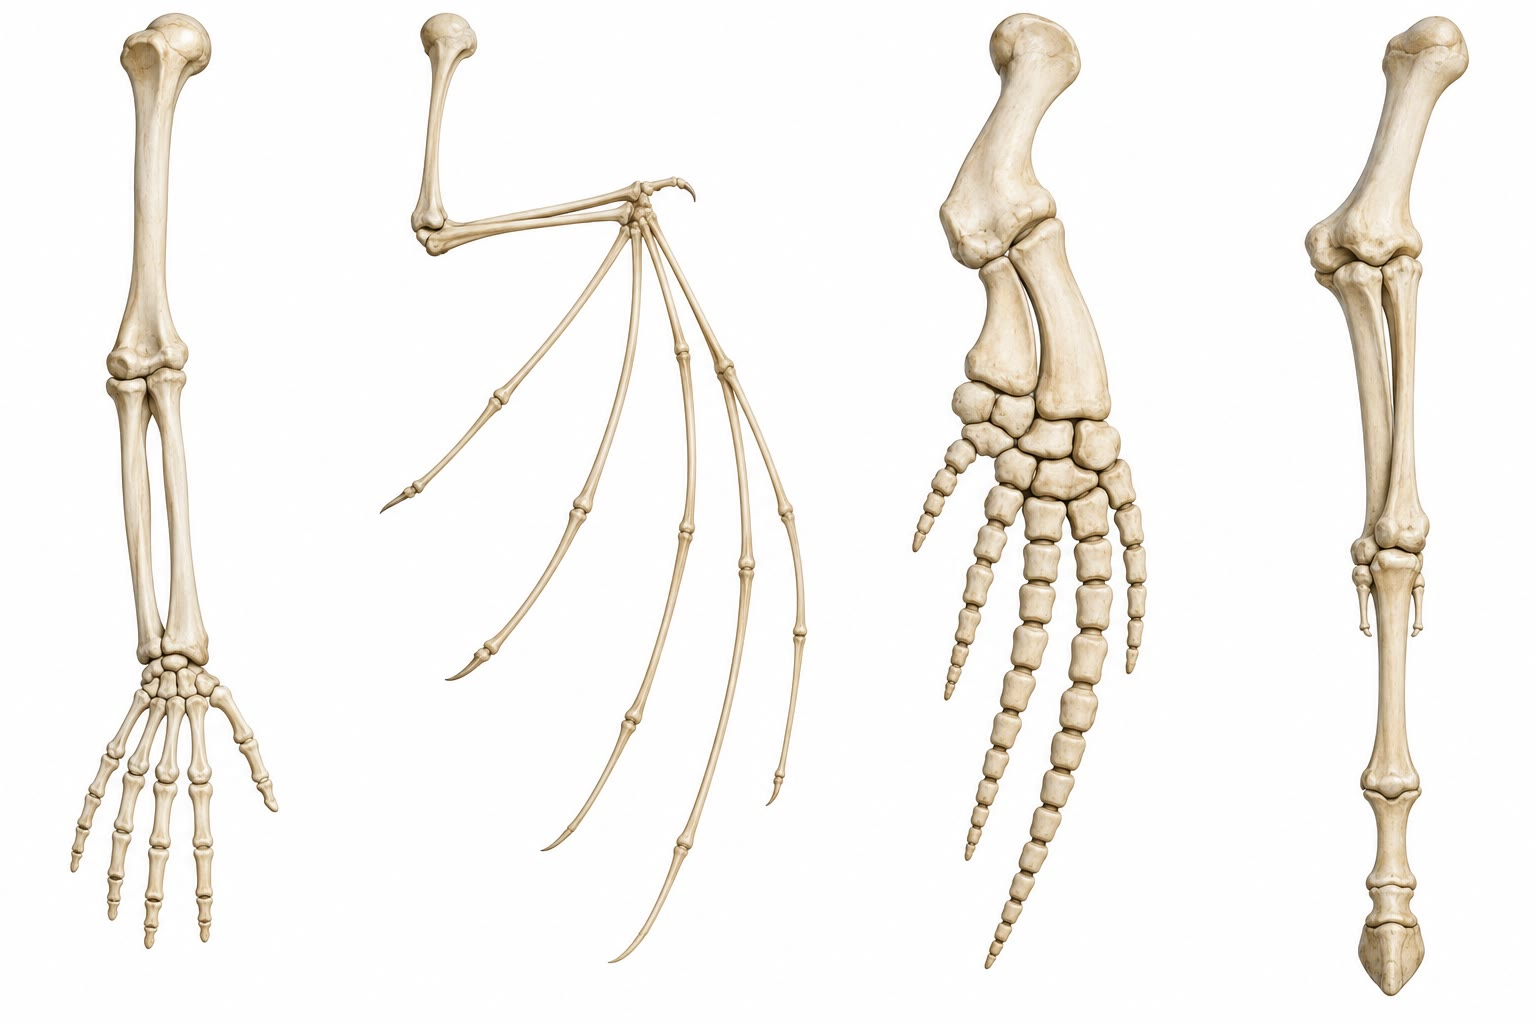
\includegraphics[width=0.44\linewidth]{images/book4/ai/b4-24-homologous-forelimbs.jpg}\hspace{0.04\linewidth}
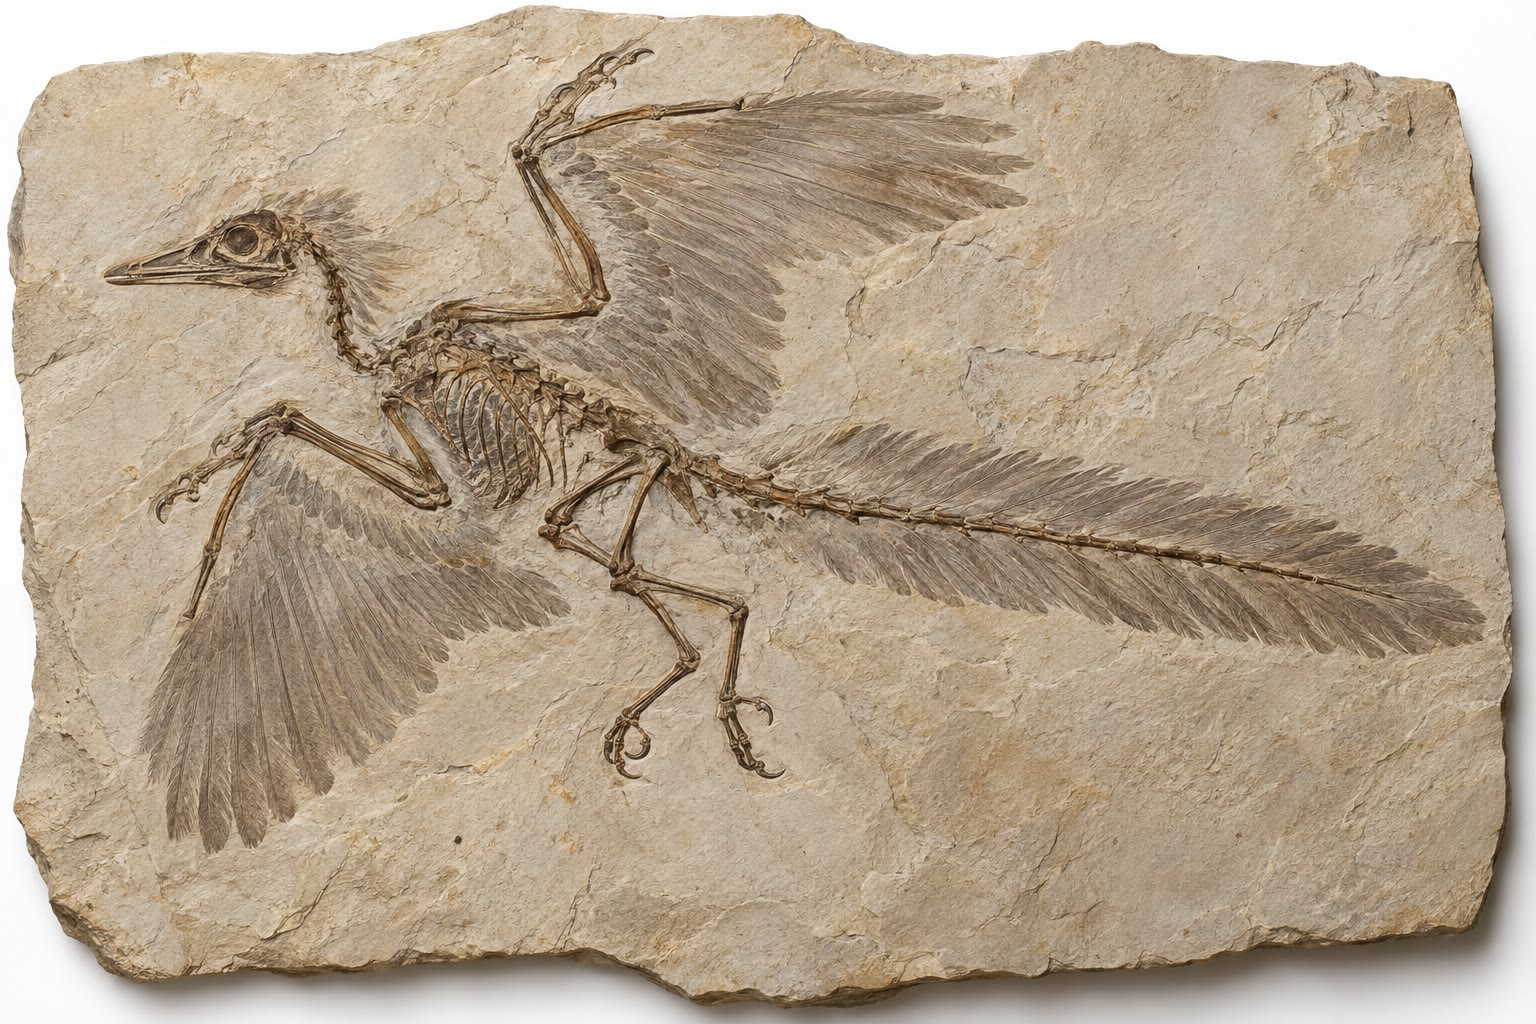
\includegraphics[width=0.44\linewidth]{images/book4/ai/b4-24-archaeopteryx.jpg}

{\small \omterm{def:b2:phylogenetic-trees:tree}{समजातता} और उसका अभिलेख। बाएँ: वही हड्डियाँ --- प्रगंडिका,
बहिःप्रकोष्ठिका तथा अंतःप्रकोष्ठिका, कलाई, पाँच अंगुलियाँ --- किसी बाँह, किसी पंख, किसी फ़्लिपर
और किसी टाँग में। दाएँ: \emph{Archaeopteryx}, जिसके दाँत, पंजेदार
अंगुलियाँ तथा लंबी अस्थिल पूँछ किसी छोटे डायनासोर की हैं और पंख किसी
पक्षी के।}
\end{omfigure}

\section{लक्षणों से वृक्ष बनाना}

\begin{method}[मितव्ययिता]\label{meth:b2:phylogenetic-trees:parsimony}
\index{मितव्ययिता}\index{बाह्यसमूह}\index{बूटस्ट्रैप}
हर वर्गक के लिए वे लक्षण (आकारिकीय दशाएँ या पंक्तिबद्ध
अनुक्रम-स्थान) अंकित कीजिए। हर संभव वृक्ष के लिए उस पर उन आँकड़ों को समझाने भर को
ज़रूरी लक्षण-परिवर्तनों की न्यूनतम संख्या गिनिए;
सबसे मितव्ययी वृक्ष को सबसे कम चाहिए। उस वृक्ष को किसी
\emph{बाह्यसमूह} से मूलित कीजिए, यानी ऐसे वर्गक से जो अध्ययन किए गए समूह के बाहर हो।
चूँकि $n$ वर्गकों के लिए अमूलित वृक्षों की संख्या $1\cdot 3\cdot
5\cdots(2n - 5)$ है --- चार वर्गकों के लिए तीन, दस के लिए $2\times 10^{6}$,
बीस के लिए $10^{20}$ --- इसलिए वह खोज केवल छोटे समुच्चयों के लिए
संपूर्ण है और उससे आगे अनुमानी। विश्वास
\emph{बूटस्ट्रैप} से मापा जाता है: उन लक्षणों को प्रतिस्थापन के साथ हज़ार
बार फिर से प्रतिचयित कीजिए, हर बार वह वृक्ष फिर बनाइए, और अभिलिखित कीजिए कि
हर \omterm{def:b2:phylogenetic-trees:tree}{अनुजात} कितनी बार लौटता है; और जो \omterm{def:b2:phylogenetic-trees:tree}{अनुजात} उन पुनःप्रतिचयनों के \qty{95}{\%} में मिले वह
सुसमर्थित है, और जो आधे में मिले वह नहीं।
\end{method}

\begin{example}[चार वर्गक, पाँच स्थान]\label{ex:b2:phylogenetic-trees:parsimony}
अनुक्रम $A = \mathrm{AAGCT}$, $B = \mathrm{AAGCC}$, $C =
\mathrm{GGACT}$, $D = \mathrm{GGATC}$। वृक्ष $((A,B),(C,D))$ पर
स्थान 1, 2 तथा 3 हर एक एक बार बदलते हैं (उस भीतरी शाखा पर), स्थान 4
एक बार ($\mathrm{C}\to\mathrm{T}$, $D$ में) और स्थान 5 दो बार
($\mathrm{T}\to\mathrm{C}$, $B$ में तथा $D$ में): यानी छह क़दम।
$((A,C),(B,D))$ पर स्थान 1--3 हर एक को दो परिवर्तन चाहिए, और स्थान 4 तथा 5 को
एक-एक: यानी आठ। $((A,D),(B,C))$ पर: नौ। पहला वृक्ष सबसे
मितव्ययी है, दो क़दम से; और जो तीन स्थान उसका समर्थन करते हैं वे
उसके \omterm{def:b2:phylogenetic-trees:tree}{सहअपसारी लक्षण} हैं, तथा स्थान 5 उस पर कोई समरूपता है --- यानी वही
परिवर्तन दो बार होता, जो हर असली आँकड़ा-समुच्चय में जीवन का एक तथ्य है।
\end{example}

\begin{omfigure}
\begin{tikzpicture}[every node/.style={font=\scriptsize}, line width=0.8pt]
  \foreach \x/\a/\b/\c/\d/\steps/\lab in {0/A/B/C/D/6/{$((A,B),(C,D))$ --- 6 क़दम}, 4.6/A/C/B/D/8/{$((A,C),(B,D))$ --- 8 क़दम}, 9.2/A/D/B/C/9/{$((A,D),(B,C))$ --- 9 क़दम}} {
    \begin{scope}[xshift=\x cm]
      \draw (0,1.6) node[left] {\a} -- (0.8,1.1) -- (0,0.6) node[left] {\b};
      \draw (0.8,1.1) -- (2.0,1.1);
      \draw (2.8,1.6) node[right] {\c} -- (2.0,1.1) -- (2.8,0.6) node[right] {\d};
      \node[anchor=north] at (1.4,0.2) {\lab};
    \end{scope}
  }
  \node[anchor=north] at (5.9,-0.6) {\begin{tabular}{l@{\ }ccccc} स्थान & 1 & 2 & 3 & 4 & 5 \\ \hline $A$ & A & A & G & C & T \\ $B$ & A & A & G & C & C \\ $C$ & G & G & A & C & T \\ $D$ & G & G & A & T & C \end{tabular}};
\end{tikzpicture}

{\small चार वर्गकों के लिए तीनों अमूलित वृक्ष, उनके नीचे के
पाँच-स्थान पंक्तिबद्धन के विरुद्ध अंकित। स्थान 1--3 पहले वृक्ष पर एक बार
और दूसरों पर दो बार बदलते हैं; स्थान 4 केवल एक वर्गक में बदलता है और
तय नहीं कर सकता, जबकि स्थान 5 $A$ को $C$ से जोड़ता है और इसलिए
तीसरे वृक्ष का पक्ष लेता है।}
\end{omfigure}

\section{दूरियों से वृक्ष बनाना}

\begin{method}[दूरी से गुच्छन: UPGMA]\label{meth:b2:phylogenetic-trees:upgma}
\index{UPGMA}\index{पड़ोसी-जोड़}\index{दूरी आव्यूह}
$n$ वर्गकों के बीच युग्मवार दूरियों से (प्रति स्थान भेद,
जैसा नीचे संशोधित), सबसे पास के जोड़े को किसी गुच्छ में जोड़िए जो उनकी दूरी की
आधी ऊँचाई की किसी गाँठ पर रखा जाए; उस जोड़े को उस
गुच्छ से बदल दीजिए, जिसकी हर दूसरे वर्गक से दूरी उसके
सदस्यों की दूरियों का औसत है; और तब तक दोहराइए जब तक एक ही गुच्छ बचे। परिणाम
कोई मूलित वृक्ष है जिसके सारे सिरे उसी ऊँचाई पर हैं --- वह हर शाखा पर
परिवर्तन की कोई अचल दर मान लेता है, यानी कोई \omterm{thm:b2:phylogenetic-trees:clock}{आणविक घड़ी}। जब
वंशक्रमों के बीच दरें भिन्न हों, तब वह विधि तेज़ विकसित होते
वंशक्रमों को उनका इतिहास जो भी हो साथ जोड़ देती है; \emph{\omterm{meth:b2:phylogenetic-trees:upgma}{पड़ोसी-जोड़}},
जो हर चरण पर उस जोड़े को जोड़ता है जिसका मिलन पूरे
वृक्ष को सबसे अधिक छोटा करे, कोई घड़ी नहीं मानता और बड़े आँकड़ा-समुच्चयों के लिए
मानक तेज़ विधि है।
\end{method}

\begin{example}[UPGMA]\label{ex:b2:phylogenetic-trees:upgma}
दूरियाँ (प्रति सौ स्थान भेदों में): $AB = 4$, $AC = 8$,
$AD = 10$, $BC = 8$, $BD = 10$, $CD = 6$। $A$ तथा $B$ को ऊँचाई 2 पर जोड़िए;
फिर $d(AB, C) = 8$, $d(AB, D) = 10$, $d(C,D) = 6$: $C$ तथा $D$ को
ऊँचाई 3 पर जोड़िए; और अंत में $d(AB, CD) = (8 + 10 + 8 + 10)/4 = 9$: उन
दोनों गुच्छों को ऊँचाई $4.5$ पर जोड़िए। वह वृक्ष $((A,B),(C,D))$ है, और यदि
वह दर प्रति स्थान प्रति वर्ष $10^{-9}$ प्रतिस्थापन हो तो वह मूल
$0.045/10^{-9} = 45$ मिलियन वर्ष पुराना है।
\end{example}

\begin{omfigure}
\begin{tikzpicture}[every node/.style={font=\scriptsize}, line width=0.8pt, x=1.1cm]
  \draw[->] (0,-0.4) -- (5,-0.4); \foreach \h in {0,1,2,3,4} \draw (\h,-0.5) -- (\h,-0.3) node[below=4pt] {\h};
  \node[anchor=north] at (2.5,-0.9) {गाँठ-ऊँचाई (प्रति सौ स्थान भेद)};
  % A,B join at 2, C,D at 3, root at 4.5 ; draw as rooted tree, root on the right
  \draw (0,3.0) node[left] {$A$} -- (2,3.0) -- (2,2.4) -- (0,2.4) node[left] {$B$};
  \draw (0,1.2) node[left] {$C$} -- (3,1.2) -- (3,0.4) -- (0,0.4) node[left] {$D$};
  \draw (2,2.7) -- (4.5,2.7) -- (4.5,0.8) -- (3,0.8);
  \fill (2,2.7) circle (1.5pt); \fill (3,0.8) circle (1.5pt); \fill (4.5,1.75) circle (1.5pt);
  \node[anchor=west] at (4.6,1.75) {मूल, 4.5};
  \node[anchor=south west] at (2.05,3.05) {2};
  \node[anchor=south west] at (3.05,1.25) {3};
  \node[anchor=west, align=left] at (6.2,2.4) {\begin{tabular}{c|ccc} & $B$ & $C$ & $D$ \\ \hline $A$ & 4 & 8 & 10 \\ $B$ & & 8 & 10 \\ $C$ & & & 6 \end{tabular}};
  \node[anchor=west, align=left] at (6.2,0.7) {$AB$ जोड़ने के बाद:\\ $d(AB,C) = 8$, $d(AB,D) = 10$\\ $CD$ जोड़ने के बाद: $d(AB,CD) = 9$};
\end{tikzpicture}

{\small चार वर्गकों पर UPGMA। हर गाँठ उन गुच्छों के बीच की
दूरी की आधी पर बैठती है जिन्हें वह जोड़ती है; और हर सिरा ऊँचाई शून्य पर अंत होता है, जैसा
कोई घड़ी माँगती है।}
\end{omfigure}

\section{आणविक घड़ी}

\begin{theorem}[पॉइसों प्रक्रम के रूप में प्रतिस्थापन, और बहु-आघातों का संशोधन]\label{thm:b2:phylogenetic-trees:clock}
\index{आणविक घड़ी}\index{जूक्स--कैंटर संशोधन}\index{संतृप्ति}
यदि किसी स्थान पर प्रतिस्थापन प्रति वर्ष किसी अचल दर $k$ से हों,
और स्थानों भर स्वतंत्र रूप से, तो किसी वंशक्रम पर समय $t$ में जितने
जमा हों वह माध्य $kt$ के साथ पॉइसों है, और $t$ वर्ष पहले विचलित हुए
दो वंशक्रमों को अलग करती प्रत्याशित संख्या है
\[
d = 2kt
\]
प्रति स्थान प्रतिस्थापन --- यानी वह \emph{\omterm{thm:b2:phylogenetic-trees:clock}{आणविक घड़ी}}। भिन्न स्थानों का
देखा गया अनुपात $p$ $d$ से छोटा है, क्योंकि
दो बार आघात पाया कोई स्थान अपने मूल क्षार पर लौट सकता है या संयोग से मेल खा सकता है;
और चार क्षारों के बराबर दरों से बदलने पर,
\[
p = \tfrac{3}{4}\bigl(1 - e^{-4d/3}\bigr), \qquad
d = -\tfrac{3}{4}\ln\bigl(1 - \tfrac{4}{3}p\bigr),
\]
यानी \emph{जूक्स--कैंटर} संशोधन। ज्यों-ज्यों $d$ बढ़ता है, $p$
$3/4$ पर संतृप्त हो जाता है --- दो यादृच्छिक अनुक्रम अपने स्थानों के एक चौथाई पर मेल खाते हैं
--- और $p \approx 0.5$ से आगे वह संशोधन हर
प्रतिचयन-त्रुटि बड़ी कर देता है: और जो जीन इतना बदल चुका हो उसने
समय रखना छोड़ दिया है। धीमे जीन (राइबोसोमी RNA, हिस्टोन) गहरी
शाखाएँ दिनांकित करते हैं, तेज़ (माइटोकॉन्ड्रियी DNA, इंट्रॉन) हाल की।
\end{theorem}
\begin{proof}
मान लीजिए $q(t)$ वह प्रायिकता है कि कोई स्थान समय $t$ के बाद भी अपना
मूल क्षार ढोता है। वह दर $k$ से खोया जाता है और, बाक़ी तीन क्षारों में से
किसी से, दर $k/3$ से फिर पाया जाता है:
$\mathrm{d}q/\mathrm{d}t = -kq + \tfrac{k}{3}(1 - q) = \tfrac{k}{3} -
\tfrac{4k}{3}q$, जिसका $q(0) = 1$ के साथ हल $q = \tfrac14 +
\tfrac34 e^{-4kt/3}$ है। कुल समय $2t$ से अलग किए गए दो वंशक्रम ---
सममिति से, वही जो $2t$ भर विकसित होता कोई एक वंशक्रम --- किसी
स्थान पर प्रायिकता $\tfrac14 + \tfrac34 e^{-4d/3}$ से मेल खाते हैं, जहाँ $d =
2kt$, इसलिए $p = 1 - q = \tfrac34(1 - e^{-4d/3})$; और उलटने पर वह
संशोधन मिलता है। वह पॉइसों गणना अचल, स्वतंत्र
घटनाओं से निकलती है, जैसे रेडियोसक्रिय क्षय की भौतिकी में, और उसका मानक
विचलन $\sqrt{kt}$ किसी भी तिथि की परिशुद्धि बाँधता है: $L$
स्थानों का कोई जीन जिसमें $dL$ प्रतिस्थापन देखे गए हों किसी विचलन को
लगभग $1/\sqrt{dL}$ की सापेक्ष परिशुद्धि तक दिनांकित करता है।
\end{proof}
\begin{proof}[प्रमाण-सामग्री]
त्सुकरकांडल और पॉलिंग (1965) ने घोड़े, मनुष्य, गाय तथा दूसरों के
हीमोग्लोबिनों के बीच भेद उनके विभाजनों की
जीवाश्म-आयुओं के समानुपाती पाए, और वह घड़ी प्रस्तावित की। फ़िच और
मार्गोलियाश (1967) ने केवल साइटोक्रोम $c$ से बीस जातियों का कोई वृक्ष
बनाया और, किसी एक ही प्रोटीन से, कशेरुकियों, कीटों तथा कवकों के
चिरपरिचित समूहन फिर पाए। विधि की निर्णायक परीक्षा
हिलिस तथा सहयोगियों का प्रायोगिक \omterm{def:b2:phylogenetic-trees:tree}{जातिवृत्त} (1992) था:
उन्होंने बैक्टीरियोफ़ाज T7 को किसी उत्परिवर्तजन के नीचे आठ वंशक्रमों की किसी ज्ञात, शाखित
शृंखला से गुज़ारा, उन उत्पादों का अनुक्रमण किया, और
वे अनुक्रम वृक्ष-निर्माण विधियों को बिना बताए दे दिए --- मितव्ययिता,
दूरी तथा संभाव्यता विधियों, सबने वह सच्चा वृक्ष फिर पाया, और
मितव्ययिता ने पैतृक अनुक्रम
\qty{98}{\%} से अधिक यथार्थता से फिर खड़े किए।
\end{proof}

\begin{omfigure}
\begin{tikzpicture}
\begin{axis}[
  width=0.7\linewidth, height=5.4cm,
  axis x line=bottom, axis y line=left,
  xmin=0, xmax=2.5, ymin=0, ymax=1.05,
  xlabel={प्रति स्थान सच्चे प्रतिस्थापन, $d$}, ylabel={देखे गए भेद, $p$},
  xlabel style={font=\small, at={(axis description cs:0.5,-0.13)}, anchor=north},
  ylabel style={font=\small},
  tick label style={font=\small}, ytick={0,0.25,0.5,0.75,1},
  legend style={font=\scriptsize, at={(0.97,0.35)}, anchor=east, draw=none},
  clip=false,
]
\addplot[very thick, omDef, domain=0:2.5, samples=80] {0.75*(1-exp(-4*x/3))};
\addlegendentry{$p = \tfrac34(1 - e^{-4d/3})$}
\addplot[thick, gray, dashed, domain=0:1.05, samples=2] {x};
\addlegendentry{$p = d$: कोई बहु-आघात नहीं}
\draw[dotted, gray] (axis cs:0,0.75) -- (axis cs:2.5,0.75); \node[font=\scriptsize, anchor=south east] at (axis cs:2.5,0.75) {संतृप्ति, $p = 3/4$};
\draw[<->, omThm, thick] (axis cs:0.383,0.30) -- (axis cs:0.383,0.383); \node[font=\scriptsize, omThm, anchor=west] at (axis cs:0.5,0.22) {$p = 0.30$ का अर्थ $d = 0.38$};
\end{axis}
\end{tikzpicture}

{\small बहु-आघात। भिन्न स्थानों का देखा गया अंश
सच्चे प्रतिस्थापनों की संख्या के साथ चढ़ता है और फिर संतृप्त हो जाता है; और कोई
कच्चा $p$ हर दूरी कम आँकता है तथा किसी वृक्ष की गहरी शाखाएँ सिकोड़ देता है।}
\end{omfigure}

\begin{proposition}[घड़ी के और वृक्षों के जाल]\label{prop:b2:phylogenetic-trees:pitfalls}
\index{लंबी-शाखा आकर्षण}\index{दर-विषमता}\index{अपूर्ण वंशक्रम-छँटाई}\index{संभाव्यता (जातिवृत्तिकी)}
वह घड़ी केवल लगभग अचल है: दरें जीनों के बीच
सौ गुना भिन्न हैं (कार्य के साथ --- हिस्टोन H4 अरब वर्ष में
दो अवशेष बदल चुका है, जबकि फ़ाइब्रिनोपेप्टाइड हर कुछ
लाख वर्ष में बदलते हैं), किसी जीन के भीतर स्थानों के बीच (तीसरे कोडॉन-स्थान,
इंट्रॉन तथा लूप सबसे तेज़ बदलते हैं), और वंशक्रमों के बीच (कृंतक
प्राइमेटों से तेज़ टिकटिकाते हैं, अपनी छोटी पीढ़ियों तथा
ऊँची उपापचय दरों के साथ)। इसलिए हर घड़ी को किसी जीवाश्म या किसी दिनांकित
भूवैज्ञानिक घटना से \emph{अंशांकन} चाहिए, और
तिथियाँ ऊपर की पॉइसों त्रुटि तथा उस अंशांकन की अपनी त्रुटि ढोती हैं।
वृक्षों के अपने जाल हैं। \emph{\omterm{prop:b2:phylogenetic-trees:pitfalls}{लंबी-शाखा आकर्षण}}: दो
वंशक्रम जो हर एक बहुत बदल चुके हों बहुत-से स्थान संयोग से
साझा करते हैं, और मितव्ययिता उनका इतिहास जो भी हो उन्हें जोड़ देती है --- और
उसका इलाज उन शाखाओं को तोड़ने के लिए सघन प्रतिचयन तथा ऐसी कोई विधि है जो वे दरें
प्रतिरूपित करे। \emph{अभिसरण} झूठे \omterm{def:b2:phylogenetic-trees:tree}{सहअपसारी लक्षण} पैदा करता है।
\emph{\omterm{prop:b2:phylogenetic-trees:pitfalls}{अपूर्ण वंशक्रम-छँटाई}}: जब जाति-उद्भव एक के बाद एक जल्दी हों तब
किसी जीन का वृक्ष उन जातियों का वृक्ष होना ज़रूरी नहीं, क्योंकि
वह पैतृक बहुरूपता हर वंशज में भिन्न ढंग से छँटती है
--- इसलिए कोई जाति-वृक्ष बहुत-से जीनों से बनाया जाता है, एक से नहीं। और
प्रोकैरियोटों में, जहाँ जीन बग़ल में चलते हैं
(\cref{ch:b2:genome-diversification}), वहाँ भिन्न जीन
भिन्न कहानियाँ कहते हैं और वह इतिहास कोई जाल है जिसमें से राइबोसोमी
जीनों का कोई वृक्ष गुज़रता है। आधुनिक व्यवहार मितव्ययिता तथा
दूरी की जगह \emph{संभाव्यता} रखता है: प्रतिस्थापन का कोई प्रतिरूप दिया हो (यानी
हर परिवर्तन की दरें, स्थानों के बीच उनकी विविधता), तो हर वृक्ष पर उसकी
शाखा-लंबाइयों समेत देखे गए अनुक्रमों की प्रायिकता गिनिए,
और वह वृक्ष चुनिए जो उन आँकड़ों को सबसे अधिक संभाव्य बनाए;
और उसका बेज़ी रूप हर \omterm{def:b2:phylogenetic-trees:tree}{अनुजात} के लिए सीधे कोई प्रायिकता देता है।
वर्ष 3 का खंड वे विधियाँ देता है; यहाँ इतना जानना काफ़ी है कि
हर वृक्ष मापे गए समर्थन वाली कोई परिकल्पना है, कोई तथ्य नहीं।
\end{proposition}
\begin{proof}[प्रमाण-सामग्री]
वोइज़ और फ़ॉक्स (1977) ने प्रोकैरियोटों भर छोटी-उपइकाई राइबोसोमी RNA
की तुलना की और मीथेनजनों को जीवाणुओं से उतना ही दूर पाया
जितना कोई भी यूकैरियोटों से है: यानी वे तीन अधिजगत, जिनकी पुष्टि तब से
अनुलेखन तथा अनुवादन मशीनरी के हर जीन ने की है, और जो
आकारिकी को अदृश्य थे। वही राइबोसोमी वृक्ष, भोलेपन से पढ़े जाएँ तो,
तेज़ विकसित होते सूक्ष्मबीजाणुओं को यूकैरियोटों के आधार पर
रख देते थे; और धीमी दरों वाले जीनों ने, तथा दर-विविधता की छूट देते प्रतिरूपों ने,
उन्हें कवकों में ले जाकर रखा, जहाँ वे हैं --- यानी
\omterm{prop:b2:phylogenetic-trees:pitfalls}{लंबी-शाखा आकर्षण} का कोई पाठ्यपुस्तकी उदाहरण, पकड़ा तथा ठीक किया गया।
\end{proof}

\begin{omfigure}
\begin{tikzpicture}[every node/.style={font=\scriptsize}, line width=0.8pt]
  \node[anchor=south] at (1.5,2.6) {सच्चा वृक्ष};
  \draw (0,2.2) node[left] {$A$} -- (0.8,1.6) -- (0,1.0) node[left] {$B$};
  \draw (0.8,1.6) -- (1.6,1.6);
  \draw[very thick, omThm] (1.6,1.6) -- (3.4,2.4) node[right] {$C$ (तेज़)};
  \draw[very thick, omThm] (0.8,1.6) -- (0.8,0.2) -- (2.6,0.2) node[right] {$D$ (तेज़)};
  \draw (1.6,1.6) -- (2.4,1.0) node[right] {$E$};
  \begin{scope}[xshift=7cm]
    \node[anchor=south] at (1.5,2.6) {वह वृक्ष जो मितव्ययिता पाती है};
    \draw (0,2.2) node[left] {$A$} -- (0.8,1.6) -- (0,1.0) node[left] {$B$};
    \draw (0.8,1.6) -- (1.6,1.6);
    \draw (1.6,1.6) -- (2.4,1.9) node[right] {$E$};
    \draw[very thick, omThm] (1.6,1.6) -- (2.2,1.0) -- (3.4,1.3) node[right] {$C$};
    \draw[very thick, omThm] (2.2,1.0) -- (3.0,0.2) node[right] {$D$};
  \end{scope}
  \node[align=center, text width=7cm] at (5.6,-1.1) {$C$ तथा $D$ हर एक बहुत-से स्थानों पर बदल चुके हैं; उनमें से एक चौथाई पर वे अब संयोग से मेल खाते हैं, जो उन्हें उनके असली संबंधियों से जोड़ते किसी भी सच्चे सहअपसारी लक्षण से अधिक है};
\end{tikzpicture}

{\small \omterm{prop:b2:phylogenetic-trees:pitfalls}{लंबी-शाखा आकर्षण}। जो दो वंशक्रम सबसे तेज़ विकसित हुए हों
वे उन संयोग-मेलों से जुड़ जाते हैं जो उनके बहुत-से परिवर्तन
पैदा करते हैं, और मितव्ययिता उन्हें सहोदर बना देती है।}
\end{omfigure}

\begin{example}[किसी जीवाश्म से दिनांकन]\label{ex:b2:phylogenetic-trees:dating}
\num{1000} स्थानों का कोई जीन गाय तथा ह्वेल के बीच उनके \qty{10}{\%} पर
भिन्न है, और जीवाश्म उनके साझा पूर्वज को 60 मिलियन
वर्ष पर रखते हैं। संशोधित करने पर, $d = -0.75\ln(1 - 0.133) = 0.107$; और वह दर $k
= d/2t = 0.107/(1.2\times 10^{8}) = 9\times 10^{-10}$ प्रति स्थान प्रति
वर्ष है। वही जीन ह्वेल तथा दरियाई घोड़े के बीच \qty{6}{\%} पर भिन्न है:
$d = 0.0625$, $t = d/2k = 35$ मिलियन वर्ष, और 62 प्रतिस्थापनों की
पॉइसों गणना से लगभग $\pm
\qty{13}{\%}$ तथा उस जीवाश्म-तिथि से कुछ और अनिश्चितता। वह आणविक परिणाम
कि ह्वेल दरियाई घोड़ों के सबसे पास के जीवित संबंधी हैं, जो 1990 के दशक में हर
शारीरिक वृक्ष के विरुद्ध इसी तरह पाया गया था, उस बताई गई दरियाई-घोड़े जैसी
टख़ना-हड्डी वाली आरंभिक ह्वेलों की खोज से पुष्ट हुआ
--- यानी वह घड़ी केवल दिनांकित नहीं करती; वह बताती है कि उन चट्टानों में क्या होना चाहिए।
\end{example}

\section{अभ्यास}

\begin{exercise}[$\star$]\label{exo:b2:phylogenetic-trees:1}
\omterm{def:b2:phylogenetic-trees:tree}{समजातता}, \omterm{def:b2:phylogenetic-trees:tree}{समवृत्तिता} तथा \omterm{def:b2:phylogenetic-trees:tree}{सहअपसारी लक्षण} की परिभाषा दीजिए, और
कशेरुकी अंगों, पंखों तथा आँखों में से हर एक का एक उदाहरण।
\end{exercise}

\begin{exercise}[$\star$]\label{exo:b2:phylogenetic-trees:2}
एकवंशीय, पारवंशीय या बहुवंशीय के रूप में वर्गीकृत कीजिए: पक्षी;
सरीसृप (पक्षियों के बिना); मछली (चतुष्पादों के बिना); उड़ने वाले
कशेरुकी; स्तनी; प्रोकैरियोट।
\end{exercise}

\begin{exercise}[$\star$]\label{exo:b2:phylogenetic-trees:3}
वृक्ष $(\text{स्तनी},(\text{कछुए},(\text{छिपकलियाँ},
(\text{मगर},\text{पक्षी}))))$ पर पक्षियों का सहोदर समूह,
स्तनियों का सहोदर समूह, और छिपकलियों तथा पक्षियों को रखता
सबसे छोटा \omterm{def:b2:phylogenetic-trees:tree}{अनुजात} बताइए। क्या मगरों तथा पक्षियों की जगहें
बदलने से वह वृक्ष बदलता है?
\end{exercise}

\begin{exercise}[$\star$]\label{exo:b2:phylogenetic-trees:4}
4, 6 तथा 10 वर्गकों के लिए कितने अमूलित वृक्ष हैं? 4 के लिए कितने
मूलित वृक्ष (हर अमूलित वृक्ष उसकी किसी भी शाखा पर मूलित किया जा
सकता है)?
\end{exercise}

\begin{exercise}[$\star\star$]\label{exo:b2:phylogenetic-trees:5}
अनुक्रम $A = \mathrm{CCTAG}$, $B = \mathrm{CCTGG}$, $C =
\mathrm{TTCAG}$, $D = \mathrm{TTCGA}$। तीनों अमूलित वृक्षों में से हर एक पर
क़दम गिनिए और सबसे मितव्ययी बताइए। उस पर कौन-से
स्थान समरूप हैं?
\end{exercise}

\begin{exercise}[$\star\star$]\label{exo:b2:phylogenetic-trees:6}
दूरियाँ (प्रति सौ स्थान): $AB = 6$, $AC = 14$, $AD = 16$,
$BC = 14$, $BD = 16$, $CD = 10$। UPGMA वृक्ष अपनी
गाँठ-ऊँचाइयों समेत बनाइए।
\end{exercise}

\begin{exercise}[$\star\star$]\label{exo:b2:phylogenetic-trees:7}
$p = 0.05$, $0.30$ तथा $0.60$ को बहु-आघातों के लिए संशोधित कीजिए। तीसरा
मान लगभग बेकार क्यों है?
\end{exercise}

\begin{exercise}[$\star\star$]\label{exo:b2:phylogenetic-trees:8}
कोई जीन प्रति स्थान प्रति वर्ष $10^{-9}$ प्रतिस्थापन से विकसित होता है। दो
जातियाँ $d = 0.02$ से भिन्न हैं: वे कब अलग हुईं? 500 मिलियन वर्ष पहले
अलग हुई दो जातियों के बीच आप कौन-सा $p$ देखेंगे,
और इस जीन से गहरे विभाजन दिनांकित करने के लिए उसका क्या अर्थ है?
\end{exercise}

\begin{exercise}[$\star\star$]\label{exo:b2:phylogenetic-trees:9}
कोई \omterm{def:b2:phylogenetic-trees:tree}{अनुजात} \num{1000} बूटस्ट्रैप पुनःप्रतिचयनों के \qty{52}{\%} में प्रकट होता है;
कोई दूसरा \qty{99}{\%} में। दोनों की व्याख्या कीजिए। पहले के बारे में
आप क्या करेंगे?
\end{exercise}

\begin{exercise}[$\star\star\star$]\label{exo:b2:phylogenetic-trees:10}
\omterm{prop:b2:phylogenetic-trees:pitfalls}{लंबी-शाखा आकर्षण} को उस संयोग-से-एक-चौथाई तर्क से समझाइए
और कहिए कि उन लंबी शाखाओं को तोड़ने वाले वर्गक जोड़ने से मदद क्यों मिलती है।
\end{exercise}

\begin{exercise}[$\star\star\star$]\label{exo:b2:phylogenetic-trees:11}
मानव तथा चिंपैंज़ी का माइटोकॉन्ड्रियी DNA स्थानों के \qty{9}{\%} पर
भिन्न है; और वह माइटोकॉन्ड्रियी दर लगभग $2\times 10^{-8}$ प्रति स्थान
प्रति वर्ष है। उस विभाजन को दिनांकित कीजिए, किसी \qty{16000}{}-स्थान
जीनोम के लिए पॉइसों अनिश्चितता दीजिए, और वे दो कारण बताइए जिनसे वह उत्तर
फिर भी दो के गुणक भर ग़लत हो सकता है।
\end{exercise}

\begin{exercise}[$\star\star\star$]\label{exo:b2:phylogenetic-trees:12}
``कोई जीन-वृक्ष कोई जाति-वृक्ष नहीं है।'' \omterm{prop:b2:phylogenetic-trees:pitfalls}{अपूर्ण
वंशक्रम-छँटाई}, क्षैतिज संचरण तथा जीन-द्विगुणन के साथ इस पर विचार कीजिए, और कहिए
कि फिर भी कोई जाति-वृक्ष कैसे पाया जाता है।
\end{exercise}

\section{समस्या: ह्वेलों का दिनांकन}

\begin{problem}[{सप्तांत समस्या --- ह्वेल, दरियाई घोड़ा, गाय, सूअर तथा
ऊँट एक जीन के लिए अनुक्रमित: वह वृक्ष मितव्ययिता से तथा
दूरी से बनाया, वह घड़ी किसी जीवाश्म पर अंशांकित, हर विभाजन अपनी
पॉइसों त्रुटि समेत दिनांकित, और वह शारीरिक वृक्ष उस आणविक से भिड़ाया गया,
और अंत ह्वेल--दरियाई घोड़ा विचलन-काल तथा उस
जीन की प्रतिस्थापन दर पर}]
\label{pb:b2:phylogenetic-trees:1}
\num{1000} स्थानों का कोई जीन ह्वेल ($W$), दरियाई घोड़े
($H$), गाय ($C$), सूअर ($P$) तथा ऊँट ($M$, यानी बाह्यसमूह) में अनुक्रमित है। भिन्न स्थानों के
देखे गए अनुपात: $WH = 0.06$; $WC = HC = 0.10$; $WP =
HP = CP = 0.12$; और $M$ तक हर दूरी $0.14$। जीवाश्म
गाय तथा ह्वेल--दरियाई घोड़ा रेखा के बीच विभाजन को 60 मिलियन वर्ष पर रखते हैं।
छह सूचनाप्रद स्थान, जिनमें ऊँट की दशा अंत में दी गई है:
\begin{center}
\begin{tabular}{l@{\quad}cccccc}
स्थान & 1 & 2 & 3 & 4 & 5 & 6 \\ \hline
$W$ & A & G & T & C & A & G \\
$H$ & A & G & T & C & G & G \\
$C$ & G & A & T & T & G & G \\
$P$ & G & A & C & T & G & A \\
$M$ & G & A & C & T & G & A \\
\end{tabular}
\end{center}

\medskip
\noindent\textbf{भाग I --- मितव्ययिता।}
\begin{enumerate}
  \item कौन-से स्थान $\{W, H\}$ के \omterm{def:b2:phylogenetic-trees:tree}{सहअपसारी लक्षण} हैं? $\{W, H,
        C\}$ के? कौन-सा स्थान सूचना नहीं देता, और कौन-सा कोई समरूपता
        या स्वअपसारी लक्षण है?
  \item उन छह स्थानों के क़दम वृक्ष
        $(M,(P,(C,(W,H))))$ पर गिनिए।
  \item उन्हें शरीर-रचनाविदों के वृक्ष $(M,(P,(W,(C,H))))$ पर गिनिए,
        जो दरियाई घोड़े को गाय के साथ सम-खुरीयों में रखता है और
        ह्वेलों को बाहर।
  \item कौन-सा वृक्ष पसंद किया जाता है, और कितने क़दमों से? वह
        अंतर कमज़ोर क्यों है, और उसे क्या मज़बूत करता?
  \item बूटस्ट्रैप उस पूरे जीन के पुनःप्रतिचयनों के \qty{83}{\%} में
        $\{W, H\}$ \omterm{def:b2:phylogenetic-trees:tree}{अनुजात} देता है। व्याख्या कीजिए।
  \item ऊँट बाह्यसमूह के रूप में क्यों काम में लिया जाता है, और उसके बजाय कोई मछली
        काम में ली जाती तो क्या ग़लत होता?
\end{enumerate}

\medskip
\noindent\textbf{भाग II --- दूरियाँ।}
\begin{enumerate}[resume]
  \item चारों भिन्न $p$ मानों ($0.06$, $0.10$, $0.12$,
        $0.14$) को बहु-आघातों के लिए संशोधित कीजिए।
  \item संशोधित दूरियों के साथ पाँचों वर्गकों पर UPGMA चलाइए और
        गाँठ-ऊँचाइयाँ दीजिए।
  \item क्या वह दूरी-वृक्ष उस मितव्ययिता-वृक्ष से सहमत है?
  \item समझाइए कि यदि ह्वेल-वंशक्रम दूसरों से दुगुना तेज़
        विकसित हुआ होता तो UPGMA क्यों चूक जाती।
  \item ह्वेल तथा दरियाई घोड़े के बीच उस जीन ने जितने प्रतिस्थापन
        जमा किए हैं वह संख्या, और उसका पॉइसों
        मानक विचलन निकालिए।
  \item उस गणना पर आधारित किसी तिथि की सापेक्ष परिशुद्धि दीजिए।
\end{enumerate}

\medskip
\noindent\textbf{भाग III --- वह घड़ी।}
\begin{enumerate}[resume]
  \item अंशांकित कीजिए: गाय--(ह्वेल, दरियाई घोड़ा) दूरी और उस
        60-मिलियन-वर्ष जीवाश्म से प्रति स्थान प्रति वर्ष दर $k$ निकालिए।
  \item ह्वेल--दरियाई घोड़ा विभाजन दिनांकित कीजिए।
  \item सूअर-विभाजन तथा ऊँट-विभाजन दिनांकित कीजिए।
  \item ह्वेल--दरियाई घोड़ा तिथि अपनी पॉइसों अनिश्चितता समेत दीजिए।
  \item वह जीवाश्म-अंशांकन स्वयं $\pm 5$ मिलियन वर्ष तक अनिश्चित है।
        उसे उस ह्वेल--दरियाई घोड़ा तिथि तक ले जाइए।
  \item कोई भिन्न, तेज़ जीन ह्वेल तथा ऊँट के बीच $p = 0.45$ देता है।
        उसे संशोधित कीजिए और इस विभाजन के लिए उसकी भरोसेमंदी पर टिप्पणी कीजिए।
\end{enumerate}

\medskip
\noindent\textbf{भाग IV --- भिड़ंत।}
\begin{enumerate}[resume]
  \item शरीर-रचनाविदों का वृक्ष उस दुहरी-घिरनी टख़ना-हड्डी पर टिका है
        जो गाय, सूअर, दरियाई घोड़े तथा ऊँट में साझा है पर जीवित
        ह्वेलों में नहीं, जिनके पश्च अंग ही नहीं हैं। समझाइए कि कोई खोया हुआ
        लक्षण ह्वेल--दरियाई घोड़ा \omterm{def:b2:phylogenetic-trees:tree}{अनुजात} के विरुद्ध क्यों नहीं गिन सकता।
  \item 2001 में पश्च अंगों वाली जीवाश्म ह्वेलें मिलीं; उनकी
        टख़ना-हड्डी में वह दुहरी घिरनी है। वह उस तर्क का क्या करता है?
  \item यदि ह्वेल सम-खुरीयों के भीतर हैं, तो क्या समूह
        ``ह्वेलों के बिना सम-खुरीय'' एकवंशीय,
        पारवंशीय या बहुवंशीय है?
  \item कोई दूसरा जीन वृक्ष $(M,(P,(H,(W,C))))$ देता है। वे दो
        कारण बताइए जिनसे कोई जीन-वृक्ष उस जाति-वृक्ष से भिन्न हो सकता है, और
        कहिए कि निर्णय कैसे किया जाए।
  \item ह्वेल तथा दरियाई घोड़े का माइटोकॉन्ड्रियी जीनोम स्थानों के
        \qty{25}{\%} पर भिन्न है। उसे संशोधित कीजिए, और प्रश्न 14 में मिली तिथि से
        माइटोकॉन्ड्रियी दर आँकिए।
  \item वह दर उस केंद्रकीय जीन की दर से इतनी ऊँची क्यों है?
  \item परिणाम बताइए: वह वृक्ष, वह केंद्रकीय दर $k$, और वह
        ह्वेल--दरियाई घोड़ा विचलन-काल अपनी अनिश्चितता समेत।
\end{enumerate}
\end{problem}
